% !TeX root = ../smc-report.tex
% !TeX encoding = UTF-8
% !TeX spellcheck = en_GB

\section*{LINFA: Smart drugs restocking}

  \subsection*{Smart drugs restocking}

    The pharmaceutical logistic chain is a very complex system, as it includes several actors and critical points (such as elevated drug costs, need for transport at monitored temperature, chance of expiration of goods, stock management, irregularity of demands, several possible logistic approaches, etc), which render the problem hard to optimize without the proper tools for decision support. In this context, possible unavailability could lead to critical situations, sometime even catastrophic, as it wouldn't be possible any more to guarantee the correct execution of one or more healthcare protocol, thus affecting the patients' health. Furthermore, orders are typically carried out on a daily basis and in a manual fashion, without the support of any decision support system. All these reasons makes restocking schedule hard, thus leading to unproductive stocks and higher stocking costs.
    
    In this scenario fits the project \textit{LINFA} (i.e. \textit{Logistica INtelligent del FArmaco}, or \textit{Smart Drug Logistic}, from Italian), that aims to develop an IT system for support to processes of drugs logistic management, in the context of healthcare or local companies. LINFA aims to increase efficiency, effectiveness and predictability of the process of drugs and medical devices restocking, within healthcare structures, through methods of predictive analysis and optimization, advanced logistic techniques and tracking features through the use of RFID technologies or the integration of healthcare and administrative information stream.
    
    For sake of simplicity, the following assumptions will be made in order to build a model:
    
    \begin{itemize}
      \item a single ward is present;
      \item the ward has a fixed number of beds (40) and a fixed maximum storage capacity (40);
      \item patients are indistinguishable;
      \item there is only one type of drug;
      \item patients can arrive through emergencies (i.e. according to a random variable) or scheduled examinations (i.e. according to a fixed constant);
      \item each day, patients can leave the ward with a certain probability;
      \item each day, patients can consume up to 3 units of drug;
      \item for each missing drug, an urgent order is issued, which arrives immediately;
      \item restock orders are issued at the end of each day and arrive immediately;
      \item the drug can be restocked in quantities of 0 (i.e. no order), 10, 20, 30 or 40.
    \end{itemize}
    
    The model in Code \ref{lst:ward} models a generic ward with the above specifications and three days of lookahead. The model is intended to characterise the evolution of the ward for the three subsequent days in order to support decision to the restock order of the current day, so it starts at the end of the current day (i.e. after patients arrival/discharge and drug consumption, but before the restock order). The arrival of patients and the consumption of drugs have been modelled through binomial distributions, as well as drug restock order choices, with different success probabilities. Sojourn time inside the ward for each patient is instead modelled through a geometric distribution.
    
    \begin{center}
      \lstinputlisting[language=prism, caption={PRISM code of the probabilistic model of a hospital ward.}, label={lst:ward}]{code/ward_dtmc.sm}
    \end{center}
    
    \question{Look at the model in Code \ref{lst:ward} and describe how it works.\\}
    \answer{
      The first thing that can be notice about the model is that it is defined as a DTMC. This is due the fact that the model is fully probabilistic (i.e. there is no non-determinism) and that the time is divided into discrete steps.
      
      In the first part of the code, before the beginning of the main module (lines 3-19), constants and probabilities are defined. Distributions for patients arrival through emergency, drug consumption and drug restock are defined as binomial distribution with different success probabilities (lines 8-11). Upper bounds of such distributions are defined as $4$ for emergency arrivals (\prism{maxER}), $3$ for drug consumption (\prism{maxConsume}) and $4$ for drug reorder choices. Arrivals of scheduled patients for the three subsequent days of lookahead are defined as fixed variables (lines 17-19). Also, cost weights are defined for the order cost of a single drug unit, the cost for urgent drug reorders and the stocking cost for keeping each drug unit in stock in the right conditions each day (lines 13-15).
      
      The main module \prism{hospitalWard} firstly defines several internal variables (lines 37-42), such as the number of hospitalised patients \prism{n}, the number of current drugs in stock \prism{stockDrugs}, the current day \prism{day}, or support variables, such as \prism{s}, \prism{tmp} or \prism{tmp2}. In particular \prism{s} is used to describe the internal state for each day of the ward.
      
      States from \prism{s=0} to \prism{s=3} (lines 31-46) are used to model the drug order for the current day and for the first and second following days. The module starts at the end of the current day (i.e. after patients arrival/discharge and drug consumption, but before the restock order) in order to include as much real information as possible from the real ward when deciding how to reorder. Lines 34-37 are used to chose probabilistically which kind of order to issue, according to the probability \prism{probOrder} defined. Lines 39-43 are then used to execute the corresponding order, effectively increasing the stocked drugs. Also, each order has a label associated, that will be used in the cost reward computation. After the order choice has been made, the \prism{day} variable is incremented and the \prism{tmp} support variable is set to the number of patients currently hospitalised, \prism{n}.
      
      States from \prism{s=10} to \prism{s=12} are used to model the arrival and discharge of patients in the ward. State \prism{s=10} (lines 49-52) of the ward is used to cycle through all the currently hospitalised patients to decide which of them will leave the ward, with probability \prism{probExit}. In this scenario the \prism{tmp} variable is used to cycle through all the patients. State \prism{s=11} (lines 55-57) is used to model the arrival of scheduled patients, the exact number of which is indicated by three constants. State \prism{s=12} (lines 60-63) instead is used to model the arrival of new patients through emergencies, modelled through a binomial distribution with success probability \prism{probER} defined.
      
      State \prism{s=20} is used to model drug consumption by the currently hospitalised patients. A binomial distribution with success probability \prism{probConsume} is used and a cycle is implemented through the use of the \prism{tmp} (lines 66-69). On top of that, for each patient, if after the drug consumption some drugs result to be missing (i.e. some drug was needed but there wasn't enough in stock), then the special action with label \prism{missingDrugs} is executed (line 71), which is needed to compute the correct cost reward. When drugs have been administered to all the patients (line 73) the module will then either start again (line 76) or stop definitely (line 77) in case the three following days have been completely modelled.
      
      Lastly, the only reward defined, \prism{totalCost}, is used to cumulate the total cost coming from different sources (lines 85-95). In particular, every time the consumption of drug is finished for a certain day, the remaining drugs in stock produce a cost determined by the weight \prism{costStorage} (line 86). Each time one or more drugs result missing during administration, and therefore an urgent order has to be issued, each missing drug produce a cost defined by the weight \prism{costUrgentOrder} (line 88). Regular orders also produce a cost, in particular a cost of $1$ for each drug ordered (lines 90-94).
    }
    
    \question{
      Add the following property, representing the expected \prism{totalCost} at the end of the three subsequent days:
      
      \lstinputlisting[language=prism, numbers=none]{code/totalCost.pctl}
      
      Then, create a new experiment to evaluate the best reorder strategy for wards that have different probabilities of drug consumption. For this experiment, set the probability constants \prism{probExit} and \prism{probER} to $0.5$ and $0.3$ respectively.
    }
    \answer{
      The results of the experiment, that plots the expected \prism{totalCost} after the three days for different consumption and reorder probabilities, are shown in Figure \ref{fig:totalCost_probOrder_probConsume_plot}.
    
    	\begin{figure}[h!]
    		\begin{center}
    			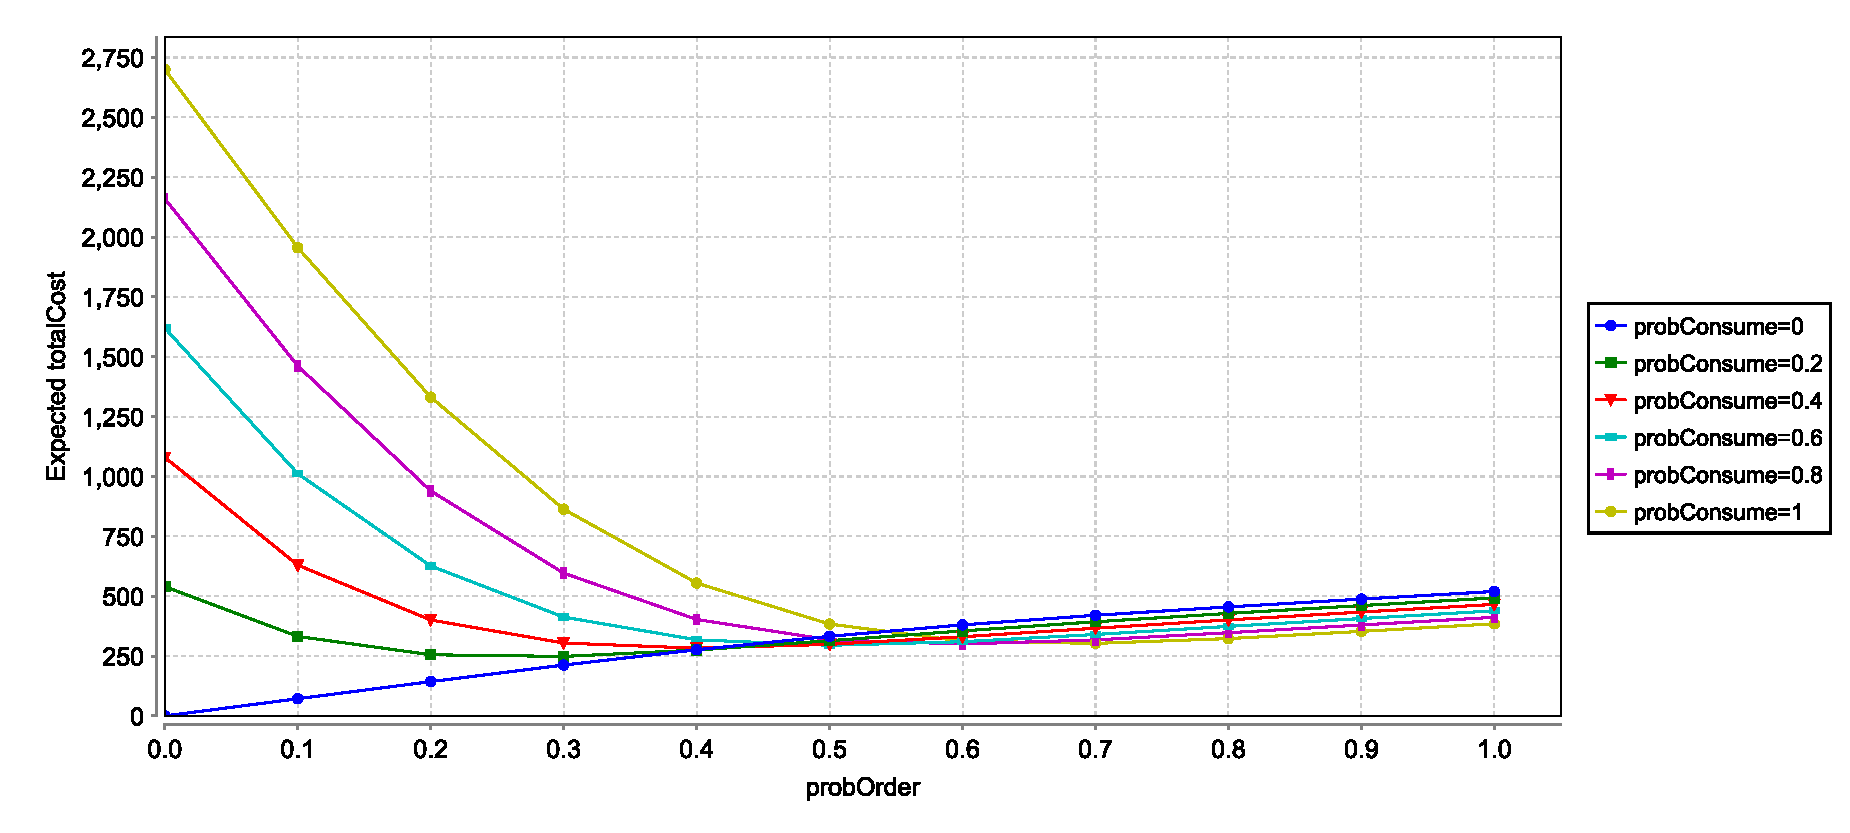
\includegraphics[scale=0.45]{totalCost_probOrder_probConsume_plot.eps}
    		\end{center}
    		\caption{Experiment plot of the expected total cost after the three subsequent days as \prism{probOrder} varies for different values of \prism{probConsume}.}
    		\label{fig:totalCost_probOrder_probConsume_plot}
    	\end{figure}
      
      As expected, lower values of \prism{probOrder} result in a higher expected \prism{totalCost} after three days for higher probabilities of consumption. This is clearly due the fact that higher consumption probabilities means a higher demand of drugs, which otherwise will deplete soon, therefore policies that tend to restock big quantities of drugs are advised in these situations. These curves, however, are not monotone, as they seem to cross around $0.6$, which seems to be also the minimum for most curves. After this point, which seems to be the best policy to be taken on average, the situation changes, meaning that higher probabilities of reordering are favoured in scenarios with higher probabilities of consumption. It is also worth noticing that the curve relative to \prism{probConsume}$=0$ is the only strictly increasing, due to the fact that if no drugs are ever consumed (i.e. never required), then reordering drugs is always just a cost and never an investment. So, as expected, low values of \prism{probConsume} requires also low values of \prism{probOrder} and viceversa. A good strategy, on average, would be to reorder with probability between $0.5$ and $0.6$.
    }
    
    \question{Perform now an experiment similar to the previous one, this time studying the best reorder strategy for wards that have different average sojourn times (i.e. probability of patient discharge). Set instead the value of \prism{probConsume} to $0.2$}
    \answer{
      The results of the experiment are shown in Figure \ref{fig:totalCost_probOrder_probExit_probConsume-0-2_plot}.
    
    	\begin{figure}[h!]
    		\begin{center}
    			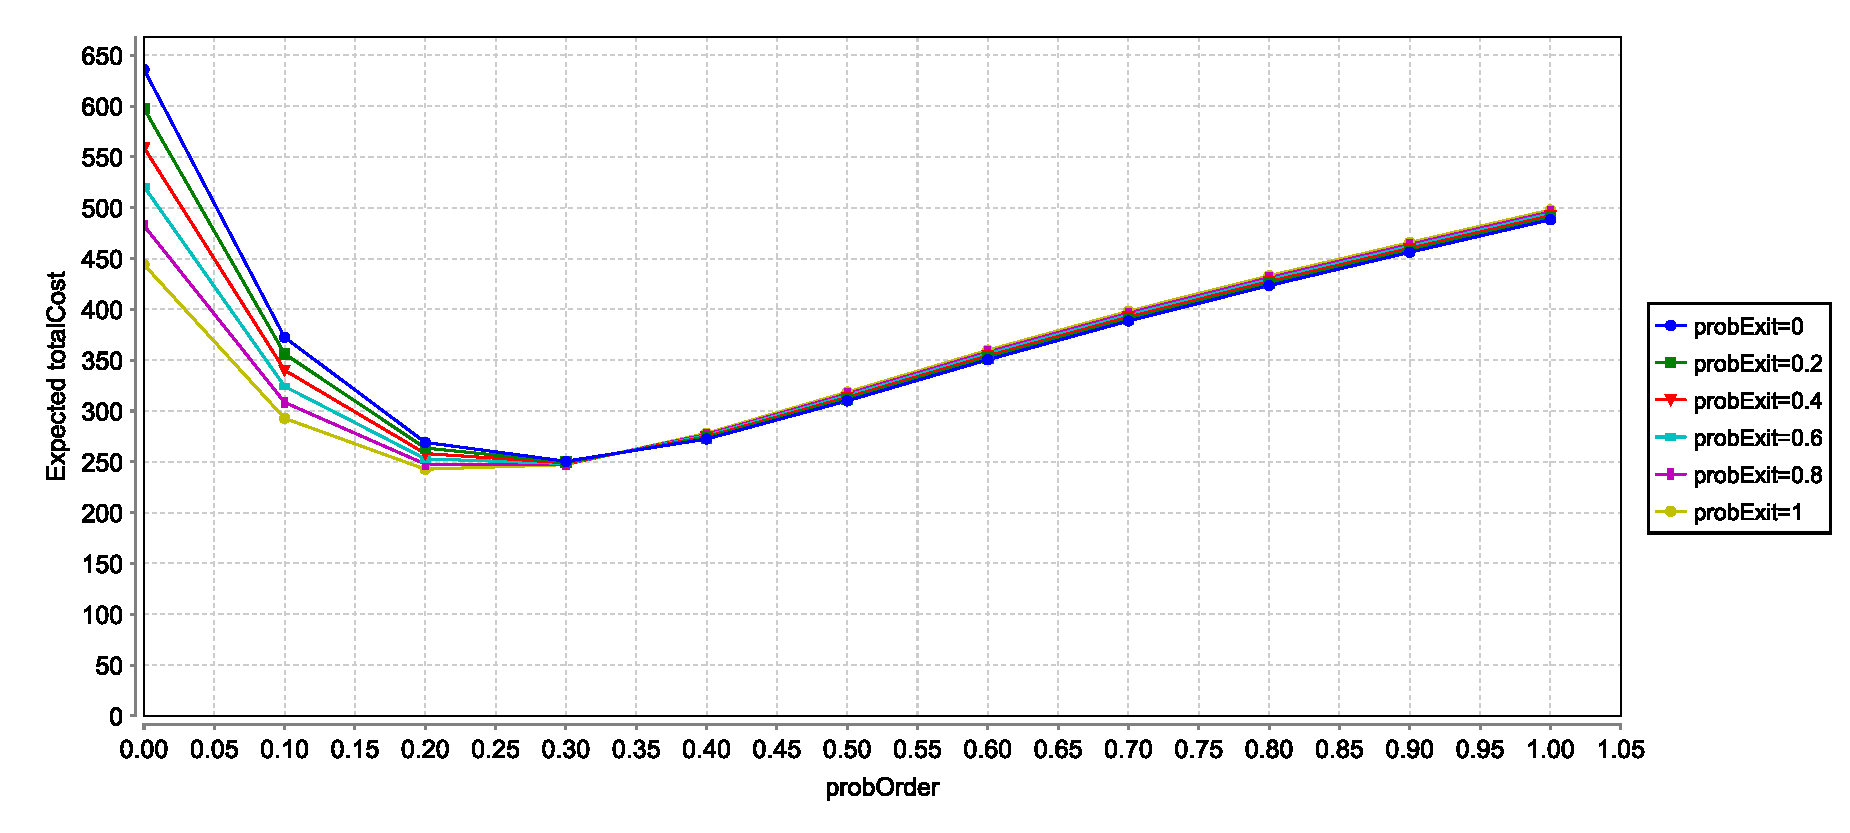
\includegraphics[scale=0.45]{totalCost_probOrder_probExit_probConsume-0-2_plot.eps}
    		\end{center}
    		\caption{Experiment plot of the expected total cost after the three subsequent days as \prism{probOrder} varies for different values of \prism{probExit}, with \prism{probConsume}$=0.2$.}
    		\label{fig:totalCost_probOrder_probExit_probConsume-0-2_plot}
    	\end{figure}
      
      The results show that, as expected, lower values of \prism{probExit} (i.e. patients stay longer, on average, in the ward) require higher values of \prism{probOrder}, while higher values of the discharge probability require a smaller reorder probability. As seen in the previous experiment, the curves cross, this time between $0.3$ and $0.35$. In this scenario, if the probability of patients discharge is unknown, the safest strategy would be with a value of \prism{probOrder} between $0.25$ and $0.3$.
    }
    
    \question{Repeat the previous experiment, this time with \prism{probConsume}$=0.8$. Which conclusions can you draw comparing the results of the two experiments?}
    \answer{
      The results of the experiment are shown in Figure \ref{fig:totalCost_probOrder_probExit_probConsume-0-8_plot}.
    
    	\begin{figure}[h!]
    		\begin{center}
    			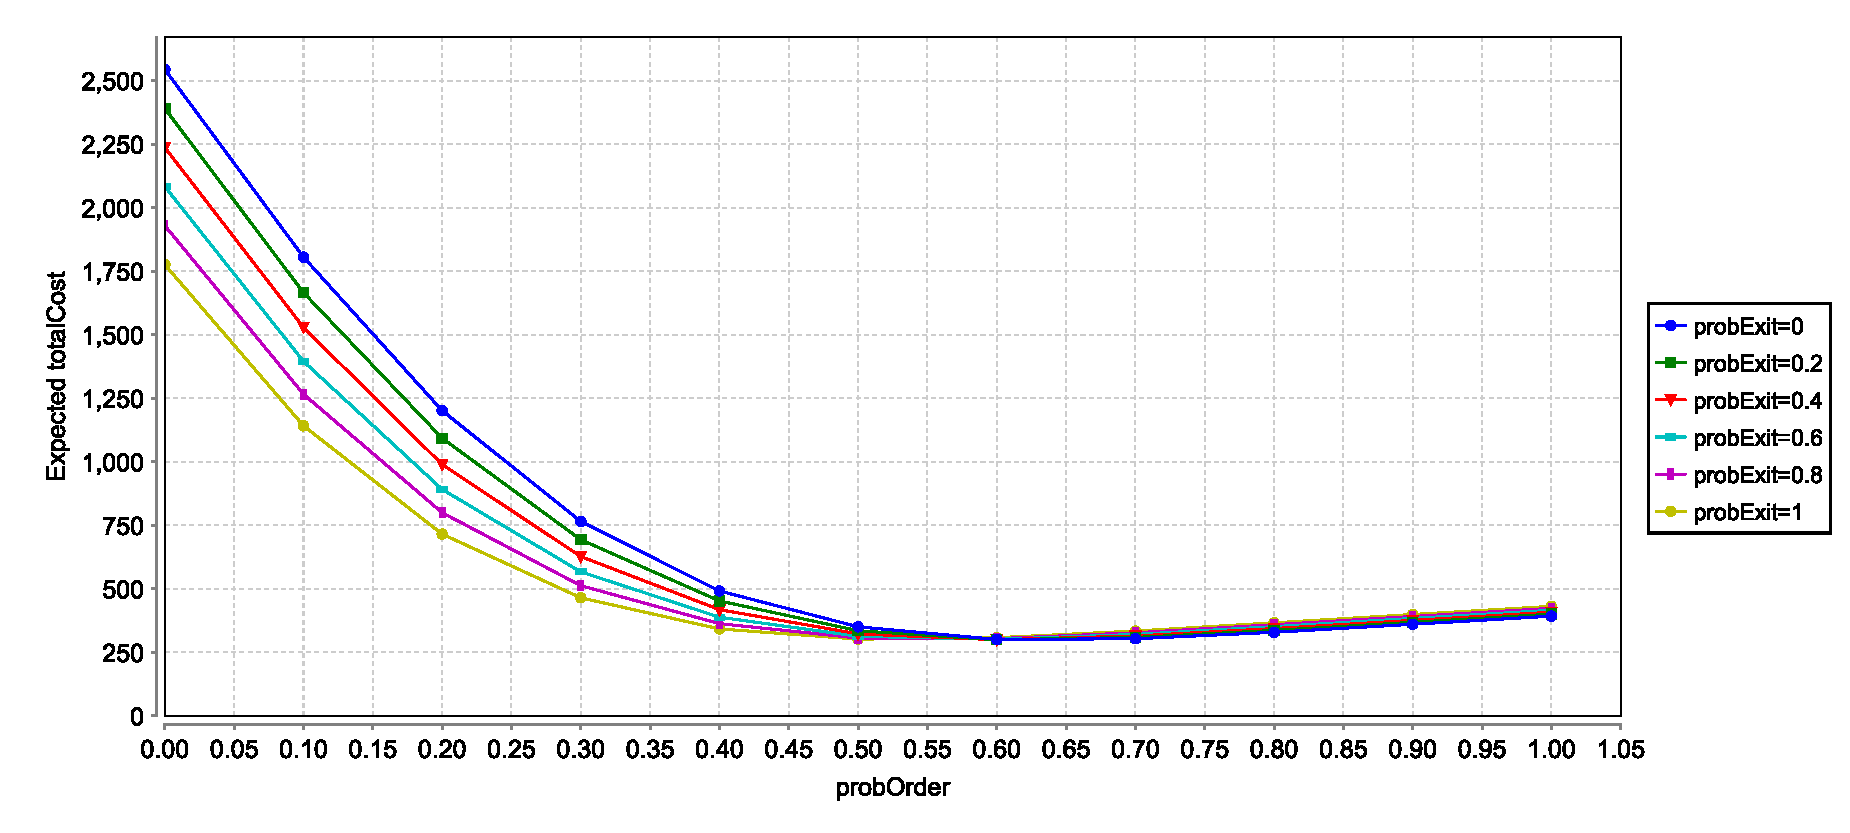
\includegraphics[scale=0.45]{totalCost_probOrder_probExit_probConsume-0-8_plot.eps}
    		\end{center}
    		\caption{Experiment plot of the expected total cost after the three subsequent days as \prism{probOrder} varies for different values of \prism{probExit}, with \prism{probConsume}$=0.8$.}
    		\label{fig:totalCost_probOrder_probExit_probConsume-0-8_plot}
    	\end{figure}
      
      The results of this last experiment are very similar to the results of the previous one, meaning that lower values of \prism{probExit} favour higher values of \prism{probOrder} and viceversa. This time, instead, the inversion point of the curves results shifted to the right, around $0.6$. This shift is due the fact that when drugs are consumed more frequently, ordering more drugs keeps being the optimal choice even if patients leave the hospital quickly, because even in the short time they spend in the ward, they are expected to consume high quantities of drugs. Also, the range of the expected \prism{totalCost} varies greatly between the two experiments: in the previous one the maximum was $636$, while for this was is $2543$. This can simply be explained by the fact that if more drugs are consumed on average, the simple cost of having to restock more drug units makes the total cost skyrocket.
    }
    
  \dashedrule
  
  \subsection*{Adding non-determinism}
    
